\documentclass[spanish, 10pt,a4paper]{article}
\usepackage[spanish]{babel}
\usepackage[utf8]{inputenc}
\usepackage{textcomp}
\usepackage{hyperref}
\usepackage[pdftex]{graphicx}
\usepackage{epsfig}
\usepackage{amsmath}
\usepackage{hyperref}
\usepackage{amssymb}
\usepackage{color}
\usepackage{graphics}
\usepackage{amsthm}
\usepackage{caratula}
\usepackage{fancyhdr,lastpage}
\usepackage[paper=a4paper, left=1.4cm, right=1.4cm, bottom=1.4cm, top=1.4cm]{geometry}
\usepackage[table]{xcolor} % color en las matrices
\usepackage[font=small,labelfont=bf]{caption} % caption de las figuras en letra mas chica que el texto
\usepackage[ruled,vlined,linesnumbered]{algorithm2e}
\usepackage{listings}
\usepackage{float}
\usepackage{amsfonts}
\usepackage{upgreek}

\color{black}

%%%PAGE LAYOUT%%%
\topmargin = -1.2cm
\voffset = 0cm
\hoffset = 0em
\textwidth = 48em
\textheight = 164 ex
\oddsidemargin = 0.5 em
\parindent = 2 em
\parskip = 3 pt
\footskip = 7ex
\headheight = 20pt
\pagestyle{fancy}
\lhead{Teor\'ia de la Comunicaciones - 2015 C2 - Trabajo Pr\'actico 1} % cambia la parte izquierda del encabezado
\renewcommand{\sectionmark}[1]{\markboth{#1}{}} % cambia la parte derecha del encabezado
\rfoot{\thepage}
\cfoot{}

%spaced sections



%El siguiente paquete permite escribir la caratula facilmente
\hypersetup{
  pdftitle={ 1c2015.PLP.RTP3},
  colorlinks,
  citecolor=black,
  filecolor=black,
  linkcolor=black,
  urlcolor=black 
}

\materia{Teor\'ia de las Comunicaciones}

\titulo{Trabajo Pr\'actico 1}

\subtitulo{Teor\'ia de las Comunicaciones}

\grupo{Grupo 4}

\integrante{Ignacio Niesz}{722/10}{ignacio.niesz@gmail.com}
\integrante{Leandro Vega}{698/11}{leandrogvega@gmail.com}
\integrante{Rodrigo Cisneros}{920/10}{rodricis@hotmail.com}
\integrante{Santiago Pernigotti}{870/11}{s.a.pernigotti89@gmail.com}
 
\begin{document}
{ \oddsidemargin = 2em
	\headheight = -20pt
	\maketitle	
}
  
	\tableofcontents
	\newpage
	\section{Introducci\'on}

	\newpage
	\section{Experimentaci\'on 1}

\subsection{Red de Starbucks}

\subsubsection{Descripci\'on del contexto}
El experimento fue realizado en una red p\'ublica Fibertel Zone, por medio de una conexión WI-FI, en uno de los locales de Starbucks, ubicado entre Honduras y Juan B. Justo. Dentro de la red se encuentran conectados notebooks, celulares y otros dispositivos con posibilidad de conexi\'on red de las personas que se encuentran dentro del local, adem\'as del router. El día y horario de la captura fue un Viernes a las 20hs. Dentro del local se encontraban alrededor de 20 personas.

\subsubsection{Descripci\'on de la captura}
La captura se realiz\'o por 20 minutos. Capturamos 232980 paquetes, de los cuales s\'olo 162 fueron paquetes del tipo ARP; los otros paquetes encontrados fueron IP version 6, LLC, DOD Internet Protocol (IP).

\subsubsection{An\'alisis de la captura}


%Sniff de Stratbucks, el viernes.

%Paquetes vistos: 382980

%Probabilidad de IP version 6: 0.00080421954149
%Probabilidad de ARP: 0.000832941667972
%Probabilidad de LLC: 0.00132382892057
%Probabilidad de DOD Internet Protocol (IP): 0.99703900987
%Entropia de S: 0.0337107429442

%Paquetes ARP vistos: 162

%Probabilidad de 10.251.24.169: 0.0308641975309 - Paquetes: 5
%Probabilidad de 10.251.24.168: 0.0185185185185 - Paquetes: 3
%Probabilidad de 10.251.24.170: 0.0432098765432 - Paquetes: 7
%Probabilidad de 10.251.24.1: 0.475308641975 - Paquetes: 77
%Probabilidad de 10.251.24.229: 0.0432098765432 - Paquetes: 7
%Probabilidad de 10.251.24.213: 0.0123456790123 - Paquetes: 2
%Probabilidad de 172.17.0.1: 0.0185185185185 - Paquetes: 3
%Probabilidad de 10.251.24.152: 0.0123456790123 - Paquetes: 2
%Probabilidad de 10.251.24.244: 0.0308641975309 - Paquetes: 5
%Probabilidad de 10.251.24.217: 0.0123456790123 - Paquetes: 2
%Probabilidad de 10.251.24.246: 0.00617283950617 - Paquetes: 1
%Probabilidad de 10.251.24.247: 0.00617283950617 - Paquetes: 1
%Probabilidad de 169.254.255.255: 0.0617283950617 - Paquetes: 10
%Probabilidad de 10.251.24.234: 0.0308641975309 - Paquetes: 5
%Probabilidad de 10.251.24.242: 0.00617283950617 - Paquetes: 1
%Probabilidad de 10.251.24.239: 0.0123456790123 - Paquetes: 2
%Probabilidad de 10.251.24.50: 0.166666666667 - Paquetes: 27
%Probabilidad de 10.251.24.245: 0.00617283950617 - Paquetes: 1
%Probabilidad de 172.17.44.238: 0.00617283950617 - Paquetes: 1
%Entropia de S_1: 2.79796437031

	\newpage
	
\subsection{Experimentaci\'on 2: Red de oficina}

\subsubsection{Descripci\'on del contexto}
El experimento fue realizado en una red de ámbito laboral. Se trata de una pequeña empresa de desarrollo web que cuenta con 13 empleados, los cuales utilizan una computadora de escritorio o notebook además de dispositivos móviles. La oficina cuenta con un servidor en donde mantine alojados los archivos de producción dentro de repositorios locales y donde los empleados suben modificaciones de los archivos constantemente.

\subsubsection{Descripci\'on de la captura}
Los resultados presentados a continuación se coresponden con la captura de paquetes de la red durante un intervalo de 3 horas.
Se capturó un total de 392521 paquetes, de los cuales 1715 fueron del tipo ARP.
\begin{itemize}
\item IP version 6: 3.67\%
\item ARP: 0.564\%
\item DOD Internet Protocol (IP): 95.7627%
\end{itemize}
Se puede observar que sólo se capturó 3 tipos de paquetes, de los cuales en su gran mayoría son del tipo DOD Internet Protocol (IP).
A contuniación se exhibe una comparación entre paquetes IP versión 6 y ARP, pudiendose observar que la cantidad de paquetes del tipo IP versión 6 es ampliamente mayor que la del tipo ARP.
\begin{center}
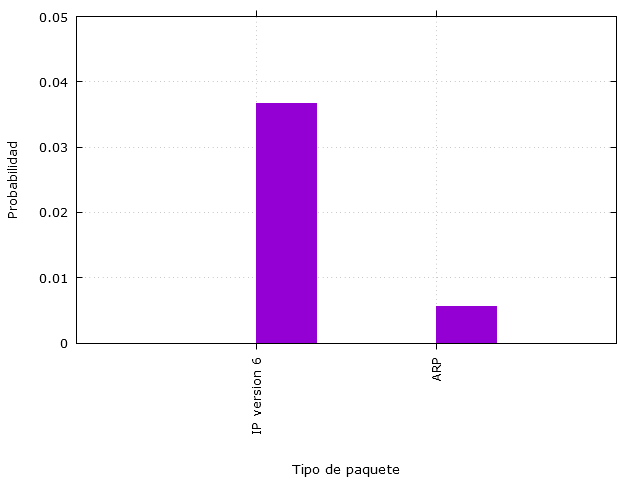
\includegraphics[width=0.5\textwidth]{exp2-graficos/grafico1exp2.png}
\end{center}

La entrop\'ia de la fuente S fue: 0.277044626815.\newline

Tomando los paquetes ARP se puede distinguir las direcciones IP en 34 diferentes, lo cual es un número razonable tiendo en cuenta la cantidad de terminales aproximada.

A continuación vemos un histograma con todas las direcciones IP observadas y la cantidad de paquetes hacia estas.

\begin{center}
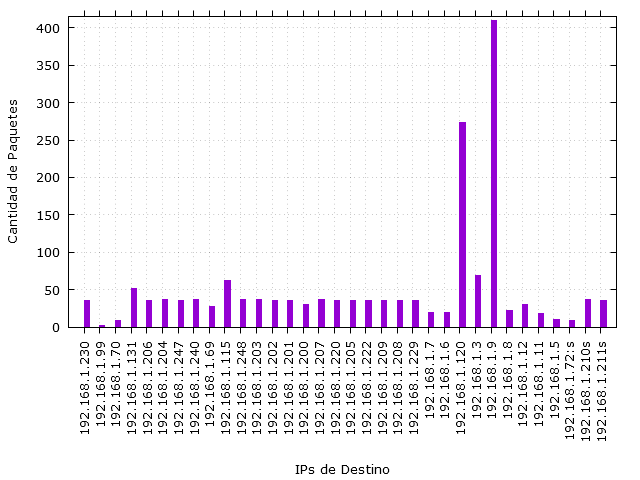
\includegraphics[width=0.75\textwidth]{exp2-graficos/grafico2exp2.png}
\end{center}

La entrop\'ia de la fuente S1 fue: 4.2739682572.


\subsubsection{An\'alisis de la captura}
Fuente $S$:
Como vimos en el 1er histograma, el 95\% de los paquetes fueron de tipo IPv4, lo que muestra que en la red hay un alto uso de paquetes de datos.

En cuanto a la entropía de la fuente es de 0.277 con lo cual se
puede ver que es más bien baja. Basandonos en la teoría de la información podemos ver que la probabilidad de un símbolo del tipo IP acapara la mayoria de la fuente, logrando que uno pueda inferir que si uno toma un símbolo emitido por la fuente este va a ser del tipo IP casi con seguridad.

Fuente $S_{1}$:
Al mirar el segundo histograma, se puede observar que las IPs más distinguidas resultan ser claramente la 192.168.1.9 y 192.168.1.120. La 192.168.1.9 resulta ser el servidor mencionado.



	\newpage
	\subsection{Experimentac\i'on 3: Red de oficina nº 2}
\subsubsection{Descripci\'on del contexto}
Usando nuestro script para analizar la red nos conectamos a una red de oficina mediante Wi-Fi. La misma es de acceso acceso restrigindo y dispone de aproximadamente de 200 terminales conectadas entre computadoras de escritorio y dispositivos m\'oviles. Al ser una oficina cuenta tanto con acces-points para conexiones de wi-fi como bocas para conexi\'on a los switches.

\subsubsection{Descripci\'on de la captura}
La captura se realiz\'o por el lapso de una hora, logrando capturar 196.495 paquetes, de los cuales 7.418 fueron de tipo ARP. Se encontraron paquetes de los siguientes tipos:

\begin{itemize}
\item LLC: 75 \%
\item IP version: 15 \%
\item ARP 3: \%
\item IP version 6: 3 \%
\item 0x5f4, 0x5e0, 0x888e: 4 \% (paquetes desconocidos en total)
\end{itemize}
En este histograma podemos ver la distribuci\'on de los distintos tipos de paquetes observados. \\

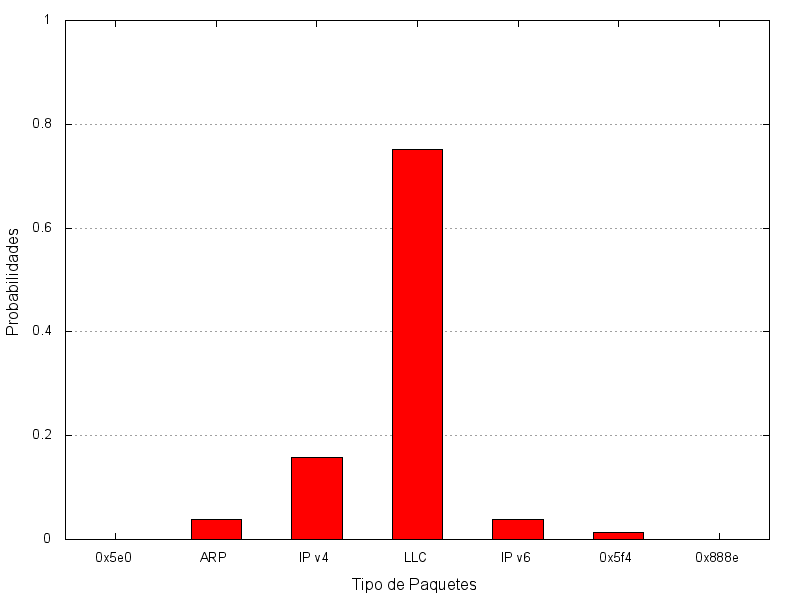
\includegraphics[scale=0.7]{exp3-graficos/s0_oficina_is.png}

En esta muestra caben destacar por un lado la inmensa cantidad de paquetes ''LLC'' en comparaci\'on al resto y los n\'umeros de paquetes desconocidos que en total superan tanto a los paquetes ARP como a los paquetes IP version 6 por separado. \\

Tomando los paquetes ARP vimos m\'as de 90 direcciones IP distintas, lo cual parece un n\'umero particularmente bajo para el tamaño de y carga de trabajo de la red.\\

Aqui vemos un gr\'afico de barras de las IP m\'as significativas de la captura, agrupadas por la presencia que tuvieron.  \\

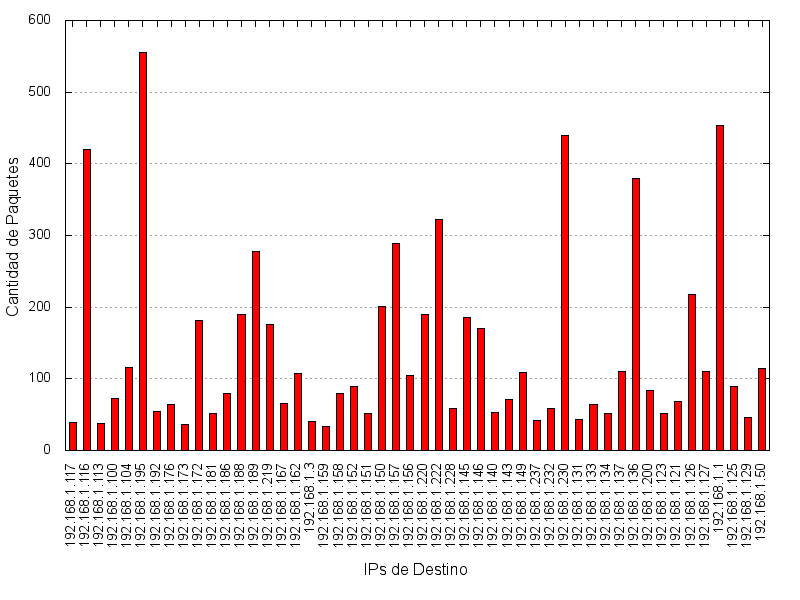
\includegraphics[scale=0.7]{exp3-graficos/s1_oficina_is_pkg.png}

Finalmente las entrop\'ias de nuestras fuentes $S$ y $S_{1}$ fueron 1.1794204458 y 5.47079616204 respectivamente.\\



\subsubsection{An\'alisis de la captura}
El an\'alisis de \'esta de los datos arrojados por la primera fuente generan las siguientes observaciones:

\begin{itemize}
\item LLC es un pr\'otocolo distinguido que supera ampliamente a IPv4/6 y ARP.
\item Tipos de paquetes desconocidos que en total superan a la cantidad de IPV4/6 y ARP por separado.
\end{itemize}

Como vimos en el 1er histograma el 75\% de los paquetes sniffeados desde la terminal conectada por wi-fi son de tipo LLC (Logical Link Control) este paquete es propio del estandard IEEE 802.2 que define el control de enlace l\'ogico para redes de \'area local en el modelo OSI. Este pr\'otocolo se encuentra en la parte superior de la capa de datos y se encarga de manejar los mecanismos de multiplexaci\'on que permite a multiples protocolos coexistir en la misma red. Adem\'as se encarga del control de flujo y de la repetici\'on de requests para manejo de errores. \\\

Actualmente este pr\'otocolo ha ca\'ido en desuso y fue reemplazado por otros como TCP que toman la responsabilidad del flujo y control de errores desde la capa de transporte. Los paquetes LLC contienen en sus headers la informaci\'on de que hacer con un paquete una vez que su frame fue recibido. \\\

Una red con 75\% de participaci\'on de paquetes LLC nos sugiere que la red local es una red de multipunto, que los nodos compiten por el uso de la misma y que se utiliza LLC para que coexistan multiples protocolos de red en un mismo medio (ej: IP, IPX, Decnet and Appletalk). \\\

El segundo punto respecto a la cantidad de paquetes desconocidos puede hacer referencia a paquetes que son recibidos con errores producto del medio de propagaci\'on. \\\


El an\'alisis de los datos arrojados por la segunda fuente nos permiten teorizar sobre los nodos distuinguidos: \\\

Observemos que de un total de m\'as de 7.400 paquetes ARP y m\'as de 90 IP's destino involucradas, el 45\% del destino de esos paquetes fue a parar \'unicamente a un 10\% de las IP's.

\begin{itemize}
\item Probabilidad de 192.168.1.195: 0.0748180102453 - Paquetes: 555
\item Probabilidad de 192.168.1.1: 0.061202480453 - Paquetes: 454
\item Probabilidad de 192.168.1.230: 0.0591803720679 - Paquetes: 439
\item Probabilidad de 192.168.1.116: 0.0566190347803 - Paquetes: 420
\item Probabilidad de 192.168.1.136: 0.0512267457536 - Paquetes: 380
\item Probabilidad de 192.168.1.222: 0.0435427338905 - Paquetes: 323
\item Probabilidad de 192.168.1.157: 0.0389592882178 - Paquetes: 289
\item Probabilidad de 192.168.1.189: 0.0373416015098 - Paquetes: 277
\item Probabilidad de 192.168.1.126: 0.0292531679698 - Paquetes: 217
\end{itemize}

Estos 9 nodos son candidato a nodos distinguidos de la red.

	\newpage
	\section{Experimentaci\'on 4}

	\newpage

\end{document}

